\subsection{Đề 2}
\Opensolutionfile{ans}[ans/ans-0-B15]
\caulc
%%==========Câu 1
\begin{ex}%[2D1N1-1]
	Cho hàm số $ y=f(x) $ liên tục trên $\mathbb{R}$ và có đạo hàm $ f'(x)=x+1 $. Hàm số đã cho nghịch biến trên khoảng nào dưới đây?
	\choice
	{\True $ (-\infty;-1) $}
	{$ (-\infty;1) $}
	{$ (-1;+\infty) $}
	{$ (1;+\infty) $}
	\loigiai{Ta có $ f'(x)<0\Leftrightarrow x+1<0\Leftrightarrow x<-1 $.\\
	Vậy hàm số $ y=f(x) $ nghịch biến trên khoảng $ (-\infty;-1) $.}
\end{ex}

%%==========Câu 2
\begin{ex}%[2D1N2-2]
	\immini{Cho hàm số $y=f(x)$ xác định, liên tục trên đoạn $[-2;2]$
	và có đồ thị là đường cong trong hình vẽ bên. Hàm số $f(x)$ đạt cực đại tại điểm nào dưới đây?
	\choice
	{$x=2$}
	{\True $x=-1$}
	{$x=1$}
	{$x=2$}
	}
	{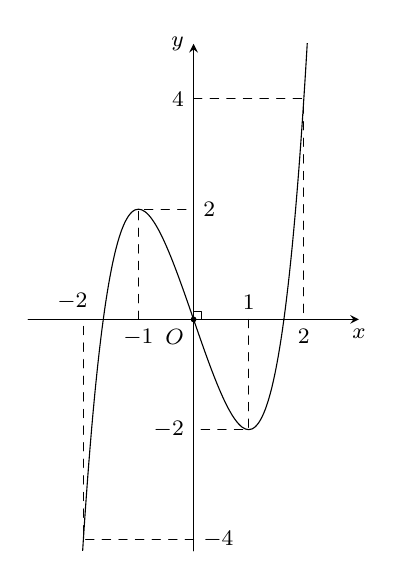
\begin{tikzpicture}[>=stealth,line join=round,line cap=round,font=\footnotesize,scale=.7]%x=2cm,y=2cm
			%========================
			\draw[->] (-3,0)--(3,0)node[below]{$x$};
			\draw[->] (0,-4.2)--(0,5)node[left]{$y$};
			\fill (0,0)node[below left]{ $O$};
			\draw (.15,0)|-(0,.15);\fill (.15,.15) circle(0pt); 
			\clip(-3,-4.2) rectangle (3,5);
			\draw[smooth,samples=100,domain=-3:3] plot(\x,{1/9*(\x)^5+7/9*(\x)^3-26/9*(\x)});
			\draw[dashed] (0,-4) -- (-2,-4) -- (-2,0);
			\draw[dashed] (0,4) -- (2,4) -- (2,0);
			\draw[dashed] (-1,0) -- (-1,2) -- (0,2);
			\draw[dashed] (1,0) -- (1,-2) -- (0,-2);
			\fill (0,0) circle (1.5pt);
			\draw(-1,0)  node[below]{$-1$}; 
			\draw(1,0)  node[above]{$1$}; 
			\draw(-2.2,0)  node[above]{$-2$}; 
			\draw(2,0)  node[below]{$2$};
			\draw(0,-2)  node[left]{$-2$}; 
			\draw(0,2)  node[right]{$2$};
			\draw(0,4)  node[left]{$4$};
			\draw(0,-4)  node[right]{$-4$};
			%========================
		\end{tikzpicture}
}
	\loigiai{
	Quan sát đồ thị, dấu $f'(x)$ đổi từ dương sang âm khi qua điểm $x=-1$ nên hàm số $f(x)$ đạt cực đại tại điểm $x=-1$.}
\end{ex}

%%==========Câu 3
\begin{ex}%[2D1H3-1]
	Giá trị nhỏ nhất của hàm số $f\left(x\right)=x^3-21x$ trên đoạn $\left[2;19\right]$ bằng
	\choice
	{$-36$}
	{\True $-14\sqrt 7 $}
	{$14\sqrt 7 $}
	{$-34$}
	\loigiai{
	Xét trên đoạn $\left[2;19\right]$ hàm số liên tục.\\
	Ta có $f'\left(x\right)=3x^2-21$.\\ Cho $f'\left(x\right)=0\Rightarrow 3x^2-21=0\Leftrightarrow\hoac{&
	x=\sqrt 7\in\left[2;19\right]\\&
	x=-\sqrt 7\notin\left[2;19\right].
	}$\\
	Khi đó $f\left(2\right)=-34$, $f\left(\sqrt 7\right)=-14\sqrt 7 $, $f\left(19\right)=6460$.\\
	Vậy $\min\limits_{\left[2;19\right]}f\left(x\right)=f\left(\sqrt 7\right)=-14\sqrt 7 $.}
\end{ex}

%%==========Câu 4
\begin{ex}%[2D1N5-1]
	Cho hàm số $y=f(x)$ có bảng biến thiên\\ 
	\centerline {
\begin{tikzpicture}[font=\normalsize]
	\tkzTabInit[nocadre=false,lgt=1.2,espcl=2.5,deltacl=0.6]
	{$x$ /0.7, $f'(x)$ /0.7, $f(x)$ /2}
	{$-\infty$, $ -1 $, $ 1 $, $ +\infty $}
	\tkzTabLine{,+,0,-,0,+,}
	\tkzTabVar{-/ $ -\infty $,+/ $ 2 $,-/ $ -2 $,+/ $ +\infty $}
	\end{tikzpicture}}
Bảng biến thiên đã cho là của hàm số nào sau đây?
	\choice{$ y=-x^3 +3x $}
	{\True $ y=x^3 -3x $}
	{$ y=-x^4 +2x^2 $}
	{$ y=x^4 -2x^2 $}
	\loigiai{
	Từ đồ thị ta có đây là đồ thị hàm số bậc $ 3 $ với hệ số $ a>0 $.}
\end{ex}

%%==========Câu 5
\begin{ex}%[2D1N1-1]
	\immini{Cho hàm số $y=f(x)$ có đồ thị như hình vẽ bên. Hàm số đã cho đồng biến trên khoảng nào sau đây?
	\choice
	{$(0;1)$}
	{$(-\infty;-1)$}
	{$(-1;1)$}
	{\True $(-1;0)$}
	}
	{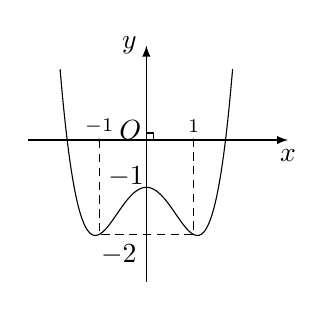
\begin{tikzpicture}[>=latex,x=1cm,y=1cm,scale=0.6]
			\draw[->] (-2.5,0)--(3,0)node[below]{$x$};
			\draw[->] (0,-3)--(0,2)node[left]{$y$};
			\fill (0.1,-.2)node[above left]{ $O$};
			\draw (.15,0)|-(0,.15);\fill (.15,.15) circle(0pt); 
			\clip(-2.5,-3) rectangle (3.2,1.5);
			\draw [thin,densely dashed] (-1,0)|-(0,-2)-|(1,0);
			\draw[smooth,samples=100,domain=-2.1:3.2] plot(\x,{3/4*(\x)^4-7/4*(\x)^2-1});
			\foreach \x in{-1,1}\draw(\x,0) circle (.5pt) node[shift={(90:5pt)}]{\scriptsize $\x$};
			\draw(0,-2) node[below left]{$-2$};
			\draw(.15,-1.2) node[above left]{$-1$};
	\end{tikzpicture}}
	\loigiai{
	Hàm số đồng biến trên các khoảng $(-1;0)$ \text{và} $(1;+\infty)$.
	}
\end{ex}

%%==========Câu 6
\begin{ex}%[2D1H2-1]
	Cho hàm số $f(x)$ có đạo hàm $f'(x)=x(x+1)(x-4)^3$, $\forall x\in \mathbb{R}$. Số điểm cực tiểu của hàm số đã cho là
	\choice
	{$4$}
	{$3$}
	{$1$}
	{\True $2$}
	\loigiai{
	Ta có $f'(x)=0\Leftrightarrow \hoac{& x=-1 \\ & x=0\\& x=4.}$\\
	Ta có bảng biến thiên như sau
	\begin{center}
	
\begin{tikzpicture}[>=stealth,scale=1]
	\tkzTabInit[lgt=1.2,espcl=2.5]
	{$x$ /0.6, $f’(x)$ /0.6, $f(x)$ /2}
	{$-\infty$,$-1$,$0$,$4$,$+\infty$}
	\tkzTabLine{,-,z,+,z,-,z,+,}
	\tkzTabVar{+/$+\infty$,-/$f(-1)$,+/$f(0)$,-/$f(4)$,+/$+\infty$}
	\end{tikzpicture}
	\end{center}
	Từ bảng biến thiên ta thấy hàm số đạt cực tiểu tại $2$ điểm $x=-1$ và $x=4$.
	}
\end{ex}

%%==========Câu 7
\begin{ex}%[2D1H3-2]
	Tính giá trị nhỏ nhất của hàm số $y=3x+\dfrac{4}{x^2}$ trên khoảng $(0;+\infty)$.
	\choice
	{\True $\min \limits_{(0;+\infty)} y=3\sqrt[3]{9}$}
	{$\min \limits_{(0;+\infty)} y=7$}
	{$\min \limits_{(0;+\infty)} y=\dfrac{33}{5}$}
	{$\min \limits_{(0;+\infty)} y=2\sqrt[3]{9}$}
	\loigiai{
	Ta có $y'=3-\dfrac{8}{x^3}=\dfrac{3x^3-8}{x^3}$; $y'=0\Leftrightarrow 3x^3-8=0 \Leftrightarrow x=\sqrt[3]{\dfrac{8}{3}}.$\\
	Ta có bảng biến thiên:\\
	\begin{center}
	
\begin{tikzpicture}
	\tkzTabInit[nocadre=false]
	{$x$ /.7, $y'$ /.7,$y$ /2}
	{$0$ ,$\sqrt[3]{\frac{8}{3}}$ , $+\infty$}
	\tkzTabLine{d,-,0,+,}% thêm d là không xác định
	\tkzTabVar{-D+/ / $+\infty$, -/$3\sqrt[3]{9}$ , + / $+\infty$}
	\end{tikzpicture}
	\end{center}
	Từ bảng biến thiên suy ra $\min \limits_{(0;+\infty)} y=3\sqrt[3]{9}.$
}
\end{ex}
%%==========Câu 8
\begin{ex}%[2D1H4-1]
	Cho hàm số $y=f(x)$ có bảng biến thiên như sau
	\begin{center}
	
\begin{tikzpicture}
	\tkzTabInit[nocadre=false, lgt=1.2, espcl=2.5,deltacl=0.6
	]{$x$ /0.6,$y'$ /0.6,$y$ /2}{$-\infty$,$1$,$+\infty$}
	\tkzTabLine{,+, d ,+,}
	\tkzTabVar{-/ $2$ / , +D-/ $+\infty$ / $3$ , +/ $5$ /}
	\end{tikzpicture}
	\end{center}
	Tổng số tiệm cận ngang và tiệm cận đứng của đồ thị hàm số đã cho là
	\choice
	{$4$}
	{$1$}
	{\True $3$}
	{$2$}
	\loigiai{
	Từ bảng biến thiên ta có
	\begin{itemize}
	\item $\lim\limits_{x \to -\infty} y =2$ suy ra $y=2$ là phương trình đường tiệm cận ngang.
	\item $\lim\limits_{x \to +\infty} y =5$ suy ra $y=5$ là phương trình đường tiệm cận ngang.
	\item $\lim\limits_{x \to 1^-} y = +\infty$ suy ra $x=1$ là phương trình đường tiệm cận đứng.
	\end{itemize}
	Vậy tổng số tiệm cận ngang và tiệm cận đứng của đồ thị hàm số đã cho là $3$.
	}
\end{ex}

%%==========Câu 9
\begin{ex}%[2D1H5-1]
	\immini{Đường cong trong hình vẽ bên là đồ thị của hàm số nào dưới đây?
	\choice
	{\True $y=x^4-2x^2-1$}
	{$y=x^4+2x^2-1$}
	{$y=x^3-x^2-1$}
	{$y=-x^3+x^2-1$}
	}
	{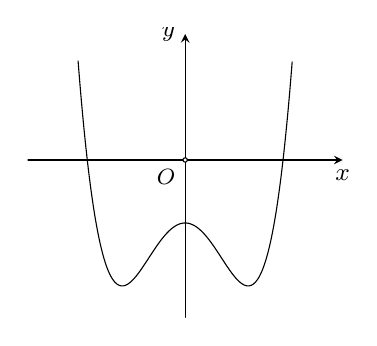
\begin{tikzpicture}[scale=.8,font=\footnotesize,line join= round,line cap=round,>=stealth,x=1cm,y=1cm]
	\clip(-2.5,-2.5) rectangle (2.6,2.1);
	\draw[->] (-2.5,0) -- (2.5,0) node[below]{\small $x$};
	\draw[->] (0,-2.5) -- (0,2.0) node[left]{\small $y$};
	\draw[smooth,samples=100,domain=-1.7:1.7] plot(\x,{(\x)^4-2*(\x)^2-1});
	\draw [fill=white] (0,0) circle (1pt)node[below left]{\footnotesize $O$};
	\end{tikzpicture}}
	\loigiai{
	Dựa vào hình dáng đồ thị ta suy ra hàm số là hàm trùng phương $ y=ax^4+bx^2+c $ có
	\begin{itemize}
	\item ``Đuôi thăng thiên'' nên $ a>0 $.
	\item Cắt trục tung tại điểm nằm phía dưới trục hoành nên $ c<0 $.
	\item Có $ 3 $ cực trị nên $ a\cdot b<0\Rightarrow b<0 $.
	\end{itemize}
	}
\end{ex}

%%==========Câu 10
\begin{ex}%[2D1H5-4]
	Số giao điểm của đồ thị hàm số $ y=x^3-x^2$ và đồ thị hàm số $ y=-x^2+5x$ là
	\choice
	{$ 2$}
	{\True $ 3$}
	{$ 1$}
	{$ 0$}
	\loigiai{
	Phương trình hoành độ giao điểm của hai đồ thị là\\
	$$x^3-x^2=-x^2+5x\Leftrightarrow{x^3}-5x=0\Leftrightarrow\hoac{
	&x=0\\
	&x=\pm\sqrt 5 .
	}$$
	Vậy số giao điểm của hai đồ thị là $ 3$.}
\end{ex}

%%==========Câu 11
\begin{ex}%[2D1V5-3]
	\immini{Cho hàm số bậc bốn $y=f\left( x \right)$ có đồ thị là đường cong trong hình bên. Số nghiệm thực phân biệt của phương trình $f\left( f\left( x \right) \right)=0$ là
	\choice
	{$12$}
	{\True $10$}
	{$8$}
	{$4$}}
	{
	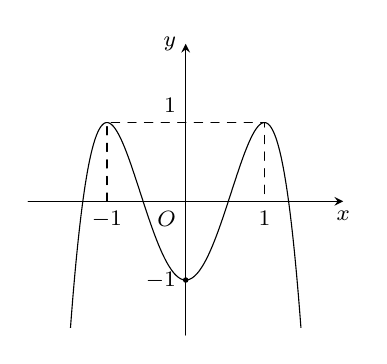
\begin{tikzpicture}[scale=1,>=stealth, font=\footnotesize, line join=round, line cap=round]
	\def\a{-2} \def\b{4} \def\c{-1} % Hệ số
	\def\xmin{-2} \def\xmax{2}
	\def\ymin{-1.7} \def\ymax{2}
	\draw[->] (\xmin,0)--(\xmax,0) node [below]{$x$};
	\draw[->] (0,\ymin)--(0,\ymax) node [left]{$y$};
	\node at (0,0) [below left]{$O$};
	\clip (\xmin+0.1,\ymin+0.1) rectangle (\xmax-0.5,\ymax-0.1);
	\draw[smooth,samples=300,domain=-2:2] plot(\x,{\a*(\x)^4+\b*(\x)^2+\c});
	\draw[dashed] (-1,0)node[below]{$-1$}|-(0,1)node[above left]{$1$}-|(1,0)node[below]{$1$};
	\fill[black] (0,-1)node[left]{$-1$} circle(1pt);
	\end{tikzpicture}
	}
	\loigiai{
	Ta có $f\left( f\left( x \right) \right)=0\Leftrightarrow \hoac{&f(x)=a\quad (a<-1) &(1) \\& f(x)=b \quad (-1<b<0)&(2) \\& f(x)=c \quad (0<c<1) &(3)\\& f(x)=d \quad (d>1).&(4)}$\\
	\immini{Từ đồ thị hàm số ta thấy
	\begin{itemize}
	\item Phương trình $\left( 1 \right)$ có $2$ nghiệm.
	\item Phương trình $\left( 2 \right)$ có $4$ nghiệm.
	\item Phương trình $\left( 3 \right)$ có $4$ nghiệm.
	\item Phương trình $\left( 4 \right)$ vô nghiệm.
	\end{itemize}
}
	{
	\begin{tikzpicture}[scale=1,>=stealth, font=\footnotesize, line join=round, line cap=round]
	\def\a{-2} \def\b{4} \def\c{-1} % Hệ số
	\def\xmin{-2} \def\xmax{2}
	\def\ymin{-2.1} \def\ymax{2.2}
	\draw[->] (\xmin,0)--(\xmax,0) node [below]{$x$};
	\draw[->] (0,\ymin)--(0,\ymax) node [left]{$y$};
	\node at ($(0,0)+(-135:2.7mm)$) {$O$};
	\draw[blue] (\xmin+0.1,1.6)--(\xmax-0.1,1.6);
	\node[blue,above,scale=0.8] at (0.8,1.53) {$y=d$};
	\fill[violet] (-1.46,-1.6) circle(1.5pt);
	\fill[violet] (1.46,-1.6) circle(1.5pt);
	\draw[blue] (\xmin+0.1,-1.6)--(\xmax-0.1,-1.6);
	\node[blue,below,scale=0.8] at (0.8,-1.55) {$y=a$};
	\draw[blue] (\xmin+0.1,0.6)--(\xmax-0.1,0.6);
	\node[blue,above,scale=0.8] at (0.37,0.53) {$y=c$};
	\fill[violet] (-1.38,-0.6) circle(1.5pt);
	\fill[violet] (1.38,-0.6) circle(1.5pt);
	\fill[violet] (-0.32,-0.6) circle(1.5pt);
	\fill[violet] (0.32,-0.6) circle(1.5pt);
	\draw[blue] (\xmin+0.1,-0.6)--(\xmax-0.1,-0.6);
	\node[blue,below,scale=0.8] at (0.85,-0.53) {$y=b$};
	\fill[violet] (-1.2,0.6) circle(1.5pt);
	\fill[violet] (1.2,0.6) circle(1.5pt);
	\fill[violet] (-0.74,0.6) circle(1.5pt);
	\fill[violet] (0.74,0.6) circle(1.5pt);
	\clip (\xmin+0.1,\ymin+0.1) rectangle (\xmax-0.5,\ymax-0.1);
	\draw[smooth,samples=300,domain=-2:2] plot(\x,{\a*(\x)^4+\b*(\x)^2+\c});
	\draw[dashed] (-1,0)node[below]{$-1$}|-(0,1)node[above left]{$1$}-|(1,0)node[below]{$1$};
	\fill[black] (0,-1)node[left]{$-1$} circle(1pt);
	\end{tikzpicture}
	}
		Vậy phương trình $f\left( f\left( x \right) \right)=0$ có tất cả $10$ nghiệm thực phân biệt.
	}
\end{ex}

%%==========Câu 12
\begin{ex}%[2D1C5-3]
	\immini{
	Cho hàm số $y=f(x)$, hàm số $y=f(x)$ liên tục trên $\mathbb{R}$ và có đồ thị như hình vẽ bên. Bất phương trình $f(x)<2x+m$ (m là tham số thực) nghiệm đúng với mọi $x \in (0;2)$ khi và chỉ khi\\
	}{
	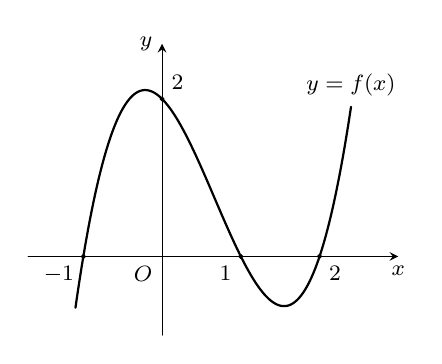
\begin{tikzpicture}[scale=1,>=stealth, font=\footnotesize, line join=round, line cap=round]
	\draw[->] (-1.7,0)--(3,0) node [below]{$x$};
	\draw[->] (0,-1)--(0,2.7) node [left]{$y$};
	\node at (0,0) [below left]{$O$};
	\draw[thick,smooth,samples=300,domain=-1.1:2.4] plot(\x,{(\x+1)*(\x-1)*(\x-2)}) node [above] {$y=f(x)$};
	\foreach \x in {-1,1}
	\draw [fill=black] (\x,0) node [below left=-0.1] {$\x$} circle (0.25mm);
	\draw [fill=black] (2,0) node [below right=-0.1] {$2$} circle (0.25mm);
	\draw [fill=black] (0,2) node [above right=-0.1] {$2$} circle (0.25mm);
	\end{tikzpicture}
	}
	\choice
	{$m>f(0)$}
	{$m>f(2)-4$}
	{\True $m \geq f(0)$}
	{$m \geq f(2)-4$}
	\loigiai{
	Ta có $f(x)<2x+m \Leftrightarrow m>f(x)-2x.\quad (1)$ \\
	Đặt $g(x)=f(x)-2x$, $x \in (0;2)$.\\
	$\forall x \in (0;2), g'(x)=f'(x)-2<0\Rightarrow$ hàm số $y=g(x)$ nghịch biến trên $(0;2)$. \\
	Do đó $(1)$ đúng với mọi $x \in (0;2)$ khi và chỉ khi $m \geq g(0)=f(0)$.}
\end{ex}
%==============================================================
\Closesolutionfile{ans}
\indapan{6}{ans/ans-0-B15}
\cauds
\Opensolutionfile{ans}[ans/ans-0-B15-DS]
%%==========Câu 13
\begin{ex}%[2D1H3-2]
	Cho hàm số $y=x^3-3x^2+1$. Xét tính đúng, sai của các khẳng định sau
	\choiceTF
	{\True Hàm số đã cho đồng biến trên khoảng $(-\infty;0)$}
	{Hàm số đã cho nghịch biến trên khoảng $(2;+\infty)$}
	{\True Giá trị cực đại của hàm số đã cho bằng $1$}
	{Giá trị nhỏ nhất của hàm số đã cho trên khoảng $(-\infty; +\infty)$ bằng $0$}
	\loigiai{
	Tập xác định $\mathscr{D}=\mathbb{R}$.\\
	Ta có $y'=3x^2-6x$.\\
	$y'=0\Leftrightarrow x=0$ hoặc $x=2$.\\
	Bảng biến thiên
	\begin{center}
	\begin{tikzpicture}
	\tkzTabInit[lgt=1.5,espcl=2,deltacl=0.5]
	{$x$/.6, $y'$/.6, $y$/1.5}
	{$-\infty$,$0$,$2$,$+\infty$}
	\tkzTabLine{,+,0,-,0,+,}
	\draw
	(N13) node[above] (A) {$-\infty$}
	(N22) node[below] (B) {$1$}
	(N33) node[above] (C) {$-3$}
	(N42) node[below] (D) {$+\infty$};
	\draw[-stealth] (A)--(B);
	\draw[-stealth] (B)--(C);
	\draw[-stealth] (C)--(D);
	\end{tikzpicture}
	\end{center}
	Từ bảng biến thiên ta thấy 
	\begin{itemchoice}
		\itemch Đúng, vì trên khoảng $(-\infty; 0)$. Hàm số đồng biến.
		\itemch Sai, vì trên khoảng $(2;+\infty)$. Hàm số đồng biến.
		\itemch Đúng, vì giá trị cực đại của hàm số bằng $1$.
		\itemch Sai, vì trên khoảng $(-\infty; +\infty)$. Giá trị nhỏ nhất của hàm số bằng $-3$.
	\end{itemchoice}
	}
\end{ex}

%%==========Câu 14
\begin{ex}%[2D1H4-1]
	Cho hàm số $y=\dfrac{x^2-4x+3}{x^4-4x^2+3}$. Xét tính đúng, sai của các khẳng định sau
	\choiceTF
	{\True Đồ thị hàm số đã cho luôn có $3$ đường tiệm cận đứng}
	{\True Đồ thị hàm số đã cho luôn có $1$ đường tiệm cận ngang}
	{ Đồ thị hàm số đã cho luôn có $5$ đường tiệm cận}
	{\True Đồ thị hàm số đã cho có $4$ đường tiệm cận}
	\loigiai{
	Tập xác định $\mathscr D=\mathbb{R}\setminus \left \{\pm 1, \pm \sqrt{3}\right \}$.\\
	Ta có $y=\dfrac{x^2-4x+3}{x^4-4x^2+3}=\dfrac{(x-1)(x-3)}{(x^2-1)\left (x^2-3\right )}=\dfrac{x-3}{(x+1)\left (x^2-3\right )}$.
	\begin{itemize}
		\item $\lim \limits_{x\to -1^+}y=+\infty; \lim \limits_{x\to -1^-}y=-\infty$. Suy ra $x=-1$ là tiệm cận đứng của đồ thị hàm số.
		\item $\lim \limits_{x\to -\sqrt{3}^+}y=-\infty; \lim \limits_{x\to -\sqrt{3}^-}y=+\infty$. Suy ra $x=-\sqrt{3}$ là tiệm cận đứng của đồ thị hàm số.
		\item $\lim \limits_{x\to \sqrt{3}^+}y=-\infty; \lim \limits_{x\to \sqrt{3}^-}y=+\infty$. Suy ra $x=\sqrt{3}$ là tiệm cận đứng của đồ thị hàm số.
		\item $\lim \limits_{x\to +\infty}y=\lim \limits_{x\to -\infty}y=0$. Suy ra $y=0$ là tiệm cận ngang của đồ thị hàm số.
	\end{itemize}
	\begin{itemchoice}
		\itemch Đồ thị hàm số đã cho luôn có $3$ đường tiệm cận đứng đúng, vì hàm số viết lại thành $$y=\dfrac{x^2-4x+3}{x^4-4x^2+3}=\dfrac{(x-1)(x-3)}{(x^2-1)\left (x^2-3\right )}=\dfrac{x-3}{(x+1)\left (x^2-3\right )}.$$
		\itemch Đồ thị hàm số đã cho luôn có $1$ đường tiệm cận ngang là đúng, vì bậc tử bé hơn bậc mẫu.
		\itemch Đồ thị hàm số đã cho luôn có $5$ đường tiệm cận là sai, vì hàm số viết lại thành $$y=\dfrac{x^2-4x+3}{x^4-4x^2+3}=\dfrac{(x-1)(x-3)}{(x^2-1)\left (x^2-3\right )}=\dfrac{x-3}{(x+1)\left (x^2-3\right )}.$$
		\itemch Đồ thị hàm số đã cho có $4$ đường tiệm cận là đúng.
	\end{itemchoice}
	}
\end{ex}

%%==========Câu 15
\begin{ex}%[2D1H5-3]
	\immini {Cho đồ thị hàm số bậc ba $y=ax^3+bx^2+cx+d$ như hình vẽ bên. Xét tính đúng, sai của các khẳng định sau
	\choiceTF
	{Đồ thị hàm số đã cho luôn nằm trên trục hoành}
	{\True Đồ thị hàm số đã cho có $2$ điểm cực trị}
	{\True Đồ thị hàm số đã cho cắt trục hoành tại $3$ điểm phân biệt}
	{\True Đồ thị hàm số đã cho có $2$ số dương trong các số $a;b;c;d$}
}
	{\begin{tikzpicture}[>=stealth,scale=0.5, line join=round, line cap=round]
			\draw[->] (-4,0)--(5.5,0)node[below]{$x$};
			\draw[->] (0,-4)--(0,4.5)node[left]{$y$};
			\draw (.15,0)|-(0,.15);\fill (.15,.15) circle(0pt); 
			\def\a{-1/5} \def\b{3/5} \def\c{9/5} \def\d{-2} % Hệ số
			\def\xt{-3} \def\xp{5} \def\yt{4} \def\yd{-3.5}
			\node at (0,0) [below left]{$O$};
			\clip (\xt-0.1,\yd+0.1) rectangle (\xp-0.1,\yt-0.1);
			\draw[smooth,samples=300] plot(\x,{\a*(\x)^3+\b*(\x)^2+\c*(\x)+\d});
	\end{tikzpicture}}
	\loigiai{
	Từ đồ thị đã cho ta thấy
	\begin{itemchoice}
		\itemch Sai, vì đồ thị hàm số đã cho luôn cắt trục hoành. 
		\itemch Đúng, vì đồ thị hàm số đã cho có $2$ điểm cực trị.
		\itemch Đúng, vì đồ thị hàm số đã cho cắt trục hoành tại $3$ điểm phân biệt.
		\itemch Đúng. Vì ta thấy $a,d<0$.\\
		Hàm số đạt $2$ tại hai điểm $x_1<0<x_2$ và $x_2>|x_1|$.\\ Ta có
		$y'=a(x-x_1)(x-x_2)=ax^2-a(x_1+x_2)x+ax_1x_2$, hay $b=-a(x_1+x_2)>0$ và $c=ax_1x_2>0$.\\
		Vậy đồ thị hàm số đã cho có $2$ số dương trong các số $a;b;c;d$.
	\end{itemchoice}
	}
\end{ex}
%%==========Câu 16
\begin{ex}%[2D1V5-3]
	\immini {Cho đồ thị hàm số bậc bốn $y = f(x)=ax^4+bx^2+c\,(a\neq 0)$ có dạng đồ thị như hình bên. Xét tính đúng, sai của các khẳng định sau	
		\choiceTF
	{\True Đồ thị hàm số đã cho có $3$ điểm cực trị}
	{\True Đồ thị hàm số đã cho cắt trục hoành tại $2$ điểm phân biệt}
	{Giá trị nhỏ nhất của hàm số trên toàn tập xác định bằng $-3$}
	{\True Phương trình $\left| f(x) \right| = \pi$ có $6$ nghiệm}
	}
	{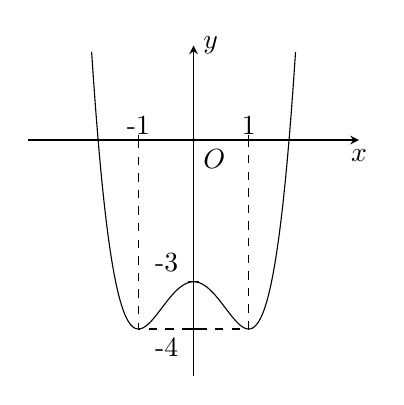
\begin{tikzpicture}[>=stealth, xscale = .7, yscale = .6]
			\draw[->] (-3,0) --(3,0)node[below]{$x$};% Trục Ok
			\draw[->] (0,-5) --(0,2) node[right]{$y$}; %Trục Ol
			\draw (0,0) node[below right]{$O$}circle(.7pt); %Điểm O
			\foreach \x in {-1,1}{\draw (\x,.1)--(\x,-.1)node[above]{\x};}
			\foreach \y in {-3}{\draw (.1,\y)--(-.1,\y)node[above left]{\y};
			}
			\foreach \y in {-4}{\draw (.1,\y)--(-.1,\y)node[below left]{\y};
			}
			\draw [domain=-1.85:1.85, samples=100] plot (\x, {(\x)^4 - 2*(\x)^2 - 3});
			\draw [dashed] (-1,0)--(-1, -4)--(0,-4)--(1,-4)--(1, 0);
			%\draw [dashed] (1,0)--(1,3)--(0,3);
		\end{tikzpicture}}
	\loigiai{
		\begin{itemchoice}
			\itemch Đúng, vì đồ thị hàm số đã cho có $3$ điểm cực trị.
			\itemch Đúng, vì đồ thị hàm số đã cho cắt trục hoành tại $2$ điểm phân biệt.
			\itemch Sai, vì giá trị nhỏ nhất của hàm số trên toàn tập xác định bằng $-4$.
			\itemch Đúng. vì ta có đồ thị của hàm số $y = \left| f(x) \right|$ có dạng như hình bên dưới.
			\begin{center}
				\begin{tikzpicture}[>=stealth, xscale = 1, yscale = .6]
					\draw[->] (-3,0) --(3,0)node[below]{$x$};% Trục Ok
					\draw[->] (0,-2) --(0,5) node[right]{$y$}; %Trục Ol
					\draw (0,0) node[below right]{$O$}circle(.7pt); %Điểm O
					\foreach \x in {-1,1}{\draw (\x,.1)--(\x,-.1)node[below]{\x};}
					\foreach \y in {4}{\draw (.1,\y)--(-.1,\y)node[above left]{\y};
					}
					\foreach \y in {3}{\draw (.1,\y)--(-.1,\y)node[below left]{\y};
					}
					\draw [domain=-1.95:1.95, samples=200] plot (\x, {abs((\x)^4 - 2*(\x)^2 - 3)});
					\draw  (-3,3.14)--(3, 3.14) node[right] {$y = \pi$};
					\draw [dashed] (-1,0)--(-1, 4)--(0,4)--(1,4)--(1, 0);
					%\draw [dashed] (1,0)--(1,3)--(0,3);
				\end{tikzpicture}
			\end{center}
			
			Từ đồ thị trên ta thấy phương trình $\left| f(x) \right| = \pi$ có $6$ nghiệm phân biệt.
		\end{itemchoice}
	}
\end{ex}
%==============================================================
\Closesolutionfile{ans}
\indapan{3}{ans/ans-0-B15-DS}
\Opensolutionfile{ans}[ans/ans-0-B15-KQ]
\caukq

%%==========Câu 17
\begin{ex}%[2D1H3-1]
	Tính giá trị nhỏ nhất của hàm số $f(x)=x^3-3x+2$ trên đoạn $[-3;3]$.
	\SA[0]{$-16$}
	\loigiai{
	$f'(x)=3x^2-3$; $f'(x)=0 \Leftrightarrow x=\pm 1 \in [-3;3]$.\\
	Ta có $f(-3)=-16$; $f(-1)=4$; $f(1)=0$; $f(3)=20$.\\
	$\Rightarrow \min\limits_{[-3;3]} f(x)=-16$.}
\end{ex}

%%==========Câu 18
\begin{ex}%[2D1H5-3]
	\immini{%
	Cho hàm số $ f(x) = ax^4 + bx^2 + c $ có đồ thị là đường cong trong hình bên. Có bao nhiêu giá trị nguyên thuộc đoạn $ \left[-2; 5\right] $ của tham số $ m $ để phương trình $ f(x) = m $ có đúng $ 2 $ nghiệm thực phân biệt?
	}{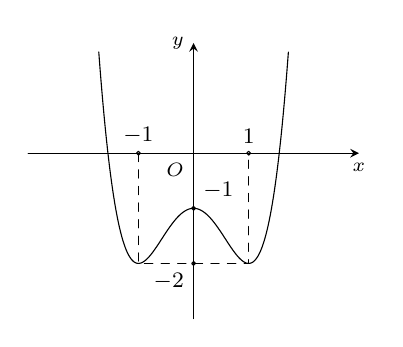
\begin{tikzpicture}[>=stealth,line join=round,line cap=round,font=\footnotesize,scale=.7]
	\def\a{1}
	\def\b{-2}
	\def\c{-1}
	\draw[->] (-3,0) -- (3,0) node[below] {\scriptsize $ x $};
	\draw[->] (0,-3) -- (0,2) node[left] {\scriptsize $ y $};
	\draw (0,0)node[below left]{\scriptsize $ O $};
	\draw[samples=150,smooth,domain=-1.72:1.72] plot(\x,{\a*(\x)^4+(\b)*(\x)^2+(\c)});
	\draw[dashed] (-1,0)--(-1,-2)--(1,-2)--(1,0);
	\draw (1,0) node[above]{$ 1 $} circle (1pt);
	\draw (-1,0) node[above]{$ -1 $} circle (1pt);
	\draw (0,-1) node[above right]{$ -1 $} circle (1pt);
	\draw (0,-2) node[below left]{$ -2 $} circle (1pt);
	\end{tikzpicture}}
	\SA[0]{$ 7 $}
	\loigiai{
	Số nghiệm phương trình $ f(x) = m $ là số giao điểm của đồ thị hàm số $ y = f(x) $ và đường thẳng $ y = m $.\\
	Suy ra phương trình $ f(x) = m $ có đúng hai nghiệm thực phân biệt $ \Leftrightarrow \left[\begin{aligned}
	& m = -2 \\
	& m > - 1.
	\end{aligned}\right. $ \\
	Do $ m \in \mathbb{Z}\Rightarrow m \in \left\{-2; 0; 1; 2; 3; 4; 5\right\} $.\\
	Vậy có $ 7 $ giá trị $ m $ thỏa mãn yêu cầu bài toán.}
\end{ex}

%%==========Câu 19
\begin{ex}%[2D1V2-3]
	Có tất cả bao nhiêu giá trị nguyên của $m$ để hàm số $$y=x^8+(m-2)x^5-(m^2-4)x^4+1$$ đạt cực tiểu tại $x=0$?
	\SA[0]{$4$}
	\loigiai{
	Ta có $y'=8x^7+5(m-2)x^4-4(m^2-4)x^3$. \\
	Đặt $g(x)=8x^4+5(m-2)x-4(m^2-4)$. Có $2$ trường hợp cần xét liên quan $(m^2-4)$:
	\begin{itemize}
	\item Trường hợp 1: $m^2-4=0 \Leftrightarrow m=\pm 2$.
	\begin{itemize}
	\item[+] Khi $m=2 \Rightarrow y'=8x^7 \Rightarrow x=0$ là điểm cực tiểu.
	\item[+] Khi $m=-2 \Rightarrow y'=x^4(8x^4-20) \Rightarrow x=0$ không là điểm cực tiểu.
	\end{itemize}
	\item Trường hợp 2: $m^2-4\ne 0 \Leftrightarrow m\ne \pm 2$. Khi đó $x=0$ không là nghiệm của $g(x)$.\\
	Ta có $x^3$ đổi dấu từ $-$ sang $+$ khi qua $x_0=0$, do đó\\
	$y'=x^3\cdot g(x)$ đổi dấu từ $-$ sang $+$ khi qua $x_0=0 \Leftrightarrow \lim\limits_{x \to 0} g(x)>0 \Leftrightarrow m^2-4<0$.
	\end{itemize}
	Kết hợp các trường hợp giải được ta nhận $m \in \{2;1;0;-1\}$.}
\end{ex}

%%==========Câu 20
\begin{ex}%[2D1V3-6]
	Các chuyên gia y tế ước tính số người nhiễm virus corona kể từ ngày xuất hiện bệnh nhân đầu tiên đến ngày thứ $t$ là $f(t)=45t^2-t^3$ với $\left(0\le t\le 25\right)$. Nếu coi $f(t)$ là một hàm xác định trên đoạn $\left[ 0;25 \right]$ thì hàm $f'(t)$ được xem là tốc độ truyền bệnh (người/ngày) tại thời điểm $t$. Xác định ngày mà tốc độ truyền bệnh là lớn nhất.
	\SA[0]{$15$}
	\loigiai{
		Từ giả thiết suy ra tốc độ truyền bệnh (người/ngày) tại thời điểm $t$ là $f'(t)=90t-3t^2$.\\
		Xét hàm $f'(t)=90t-3t^2$ với $0\le t\le 25$.\\ Ta có $f''(t)=90-6t=0\Leftrightarrow t=15$.
		\begin{center}
			
\begin{tikzpicture}
				\tkzTabInit[nocadre=false,lgt=1.2,espcl=2.5,deltacl=0.6]
				{$t$ /0.6,$f''(t)$ /0.6,$f'(t)$ /2}
				{$0$,$15$,$25$}
				\tkzTabLine{,+,0,-,}
				\tkzTabVar{-/$0$,+/$675$,-/$375$}
			\end{tikzpicture}
		\end{center}
		Từ bảng biến thiên ta có ngày mà tốc độ truyền bệnh là lớn nhất là ngày thứ $15$.
	}
\end{ex}

%%==========Câu 21
\begin{ex}%[2D1C5-4]
	Cho hàm số $y = \dfrac{x - 2}{x + 1}$ có đồ thị $\left( C \right)$. Gọi $I$ là giao điểm của hai tiệm cận của $\left( C \right)$. Xét tam giác đều $ABI$ có hai đỉnh $A$, $B$ thuộc $\left( C \right)$, đoạn thẳng $AB$ có độ dài bằng bao nhiêu? (kết quả làm tròn đến hàng phần trăm).
	\SA[0]{$3{,}46$}
	\loigiai{
	Tịnh tiến hệ trục theo véc-tơ $\overrightarrow{OI}=(-1;1)\Rightarrow I(0;0)$ và $(C)\colon Y=\dfrac{-3}{X}$.\\
	Gọi $A\left(a;\dfrac{-3}{a}\right)$, $B\left(b;\dfrac{-3}{b}\right)\in (C)$, điều kiện $a\neq b$.\\
	Tam giác $IAB$ đều
	\begin{eqnarray*}
	& \heva{& IA=IB\\&\cos(\overrightarrow{IA},\overrightarrow{IB})=\cos 60^\circ}
	\Leftrightarrow\heva{&a^2+\dfrac{9}{a^2}=b^2+\dfrac{9}{b^2}\quad (1)\\& \dfrac{ab+\dfrac{9}{ab}}{\sqrt{a^2+\dfrac{9}{a^2}}\cdot\sqrt{b^2+\dfrac{9}{b^2}}}=\dfrac{1}{2}.\quad (2)}
	\end{eqnarray*}
	Từ $(2)\Rightarrow ab>0$ do đó $(1)\Leftrightarrow (a^2-b^2)(a^2b^2-9)=0\Rightarrow ab=3$.\\
	Suy ra $AB^2=2\left(3+\dfrac{9}{3}\right)=12\Rightarrow AB=2\sqrt{3}$.
	}
\end{ex}

%%==========Câu 22
\begin{ex}%[2D1C5-3]
	Cho hàm số $y=f (x) $ có bảng biến thiên như sau
	\begin{center}
	
\begin{tikzpicture}[>=stealth,line join=round,line cap=round,font=\footnotesize,scale=1]
	\tkzTabInit[nocadre=false,lgt=1,espcl=2,deltacl=0.5]{$x$/.7 ,$y'$/.7,$y$/2}
	{$-\infty$ , $-1$ , $0$ , $1$ , $+\infty$}
	\tkzTabLine{ , - , $0$ , + , $0$ , - , $0$ , + , }
	\tkzTabVar{+/$+\infty$ , -/$-2$, +/$-1$ , -/$-2$ , +/$+\infty$}
	\end{tikzpicture}
	\end{center}
	Phương trình $2f( \sin x )+3=0$ có bao nhiêu nghiệm thuộc đoạn $\left[ -\pi ;2\pi \right]$?
	\SA[0]{$ 6 $}
	\loigiai{
	Ta có $2f\left( \sin x \right)+3=0 \Leftrightarrow f\left( \sin x \right)=-\dfrac{3}{2}$. \\
	Dựa vào bảng biến thiên của hàm số $f(x)$\\
	Do đó $f\left( \sin x \right)=-\dfrac{3}{2} \Leftrightarrow \hoac{& \sin x=t_1 \in (- \infty;-1) \\ & \sin x=t_2 \in (-1;0) \\ & \sin x =t_3 \in (0;1) \\ & \sin x =t_4 \in (1;+\infty). } $\\
	\begin{center}
	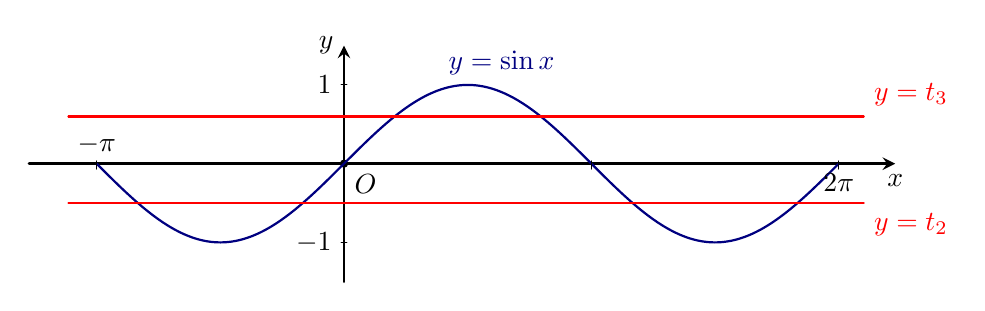
\begin{tikzpicture}[line join = round, line cap = round,>=stealth,thick,scale = 1]
	%Vẽ hệ trục Oxy
	\draw[->,line width = 1pt] (-4,0)--(0,0) node[below right]{$O$}--(7,0) node[below]{$x$};
	\draw[->,line width = 1pt] (0,-1.5)--(0,1.5) node[left]{$y$};
	\fill (0,0) circle (1.5pt);
	%Vẽ đồ thị hàm số
	\draw[samples=300,domain=-pi:2*pi,smooth,blue!50!black] plot (\x, {sin(\x r)});
	%Vẽ các điểm trên hệ trục
	\foreach \x in {-pi,pi,2*pi} \draw[thin] (\x,1pt)--(\x,-2pt);
	\foreach \y in {-1,1} \draw[thin] (1pt,\y)--(-1pt,\y) node [left] {$\y$};
	\node at (-pi,0) [above] {$-\pi$};
	\node at (2*pi,0) [below] {$2\pi$};
	\node[blue!50!black] at (2,1) [above] {$y = \sin x$};
	\draw [red]
	(-3.5,-0.5)--(6.6,-0.5)node[below right]{$ y=t_2 $}
	(-3.5,0.6)--(6.6,0.6)node[above right]{$ y=t_3 $};
	\end{tikzpicture}
	\end{center}
	\begin{itemize}
	\item Phương trình $ \sin x=t_1 $ và $ \sin x=t_4 $ vô nghiệm.
	\item Phương trình $ \sin x=t_2 $ có $ 4 $ nghiệm phân biệt.
	\item Phương trình $ \sin x=t_3 $ có $ 2 $ nghiệm phân biệt khác các nghiệm của phương trình $ \sin x=t_2 $.
	\end{itemize}
	Vậy, phương trình $2f\left( \sin x \right)+3=0$ có 6 nghiệm thuộc đoạn $\left[ -\pi \,;2\pi \right]$.
	}
\end{ex}
%==============================================================
\Closesolutionfile{ans}
\indapan{6}{ans/ans-0-B15-KQ}